% Define a counter named 'exercisecounter' to track the exercise.
% The counter will be reset to zero each time the 'chapter' counter
% is incremented (when a new chapter is created for example).
% See pandoc_filter.py3
% The same for 'projectcounter' to track projects.
\newcounter{exercisecounter}[chapter]
\newcounter{projectcounter}[chapter]

% redefine the \theCounterName macros to expand the current
% chapter number and the Counter value in arabic (like 3.2)
\renewcommand\theexercisecounter{\arabic{chapter}.\arabic{exercisecounter}}
\renewcommand\theprojectcounter{\arabic{chapter}.\arabic{projectcounter}}

\usepackage{graphicx}
\usepackage{wrapfig}

% Map Unicode emojis to PDF images. Based on coloremoji.sty
% See https://github.com/alecjacobson/coloremoji.sty
\usepackage{newunicodechar}
\newunicodechar{😈}{\text{\raisebox{-0.2em}{
\includegraphics[height=1em]{z/img/emoji/evil.pdf}}}}
\newunicodechar{💣}{\text{\raisebox{-0.2em}{
\includegraphics[height=1em]{z/img/emoji/bomb.pdf}}}}
\newunicodechar{⚠}{\text{\raisebox{-0.2em}{
\includegraphics[height=1em]{z/img/emoji/alert.pdf}}}}
\newunicodechar{↯}{\text{\raisebox{-0.2em}{
\includegraphics[height=1em]{z/img/emoji/bend.png}}}}
\newunicodechar{☣}{\text{\raisebox{-0.2em}{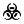
\includegraphics[height=1em]{z/img/emoji/biohazard.png}}}}

% Set language type to Spanish but allow to switch to English/Russian
% This configures the font's ligature, the predefined words "Figure"
% and "Table" (that now in Spanish will be "Figura" and "Tabla") and other
% stuff
% https://es.overleaf.com/learn/latex/Multilingual_typesetting_on_Overleaf_using_polyglossia_and_fontspec
\usepackage{polyglossia}
\setdefaultlanguage{spanish}
\setotherlanguages{english,russian}

% Set fonts
% See https://es.overleaf.com/learn/latex/XeLaTeX
% https://es.overleaf.com/learn/latex/Multilingual_typesetting_on_Overleaf_using_polyglossia_and_fontspec
% https://es.overleaf.com/learn/latex/Russian
% https://es.overleaf.com/learn/latex/Spanish
% https://www.overleaf.com/learn/latex/Articles/Unicode,_UTF-8_and_multilingual_text:_An_introduction
%
% Examples
% https://www.overleaf.com/latex/examples/how-to-write-multilingual-text-with-different-scripts-in-latex/wfdxqhcyyjxz
% https://www.overleaf.com/latex/templates/multilingual-thank-you/wjmrnnqkstyf
%
% These fonts supports bold, italics and that kind of styles
% but also supports Cyrillic (Russian) letters and mathematical
% symbols as unicode.
\usepackage{fontspec}
\setmainfont{FreeSerif}
\setsansfont{FreeSans}
\setmonofont{FreeMono}

% Font family for the code (requires calling \monacofont)
\newfontfamily\monacofont[Path=./z/fonts/]{monaco.ttf}

% Disabled because it enters in conflict with tikz
% The error says:
%
%   ! Argument of \language@active@arg> has an extra }.
%   <inserted text>
%                   \par
%   l.86 ...in{tikzpicture}[>=latex',line join=bevel,]
%\usepackage[spanish]{babel}

% Show in each page a DRAFT marker
\usepackage{draftwatermark}
\SetWatermarkColor[gray]{0.96}

% With this additional setting, the marker DRAFT is "actually" empty.
% The DRAFT word will be shown but it will be uncopyable
% https://tex.stackexchange.com/questions/309875/uncopyable-watermark
\SetWatermarkLightness{0.96}\SetWatermarkText{%
    \BeginAccSupp{method=escape,ActualText={}}DRAFT\EndAccSupp{}
}

% call \chapterauthor{aaa} *after* each chapter begin to name the author
% of it
\makeatletter
\newcommand{\chapterauthor}[1]{%
  {\parindent0pt\vspace*{-25pt}%
  \linespread{1.1}\large\scshape#1%
  \par\nobreak\vspace*{35pt}}
  \@afterheading%
}
\makeatother

\title{Guía de Taller}
\author{Martín Di Paola}

\hypersetup{
            pdftitle={Guía de Taller},
            pdfauthor={Martín Di Paola},
            pdfborder={0 0 0},
            breaklinks=true}

% Define some colors
\usepackage{xcolor}
\definecolor{darkgreen}{rgb}{0,.5,0}
\definecolor{darkblue}{rgb}{0,0,.7}

% Graph and tree diagrams
\usepackage{tikz}
\usetikzlibrary{snakes,arrows,shapes}
\usepackage{amsmath}

\usepackage{fancyvrb}

% This package allows any kind of "boxes" to put messages.
% It is used by pygmentex to put the snippets of code.
\usepackage{tcolorbox}
\tcbuselibrary{breakable}
\tcbuselibrary{skins}

% This package takes the code inside the "pygmented" (block) environments
% and the "pyginline" (inline) snippets and replaces them with the highlighted
% source code.
% This works in two passes: the first the latex is processed and the snippets
% are extracted out in a file called ".snippets". By hand someone process this
% file and generates the highlighted code and saves it into ".pygmented" file.
% This "by hand process" is done by scripts/x/pygmenter_xelatex.sh and
% ./scripts/x/pygmentex.py.
% The second pass the ".pygmented" is included back into the tex file.
%
% This package uses tcolorbox for handling the boxes where the code will be.
\usepackage{pygmentex}
\setpygmented{font=\monacofont\small,boxing method=tcolorbox,inline method=tcbox}

% Draw a tiny ruler for the code snippets.
% https://tex.stackexchange.com/questions/128636/center-hrule-in-the-middle-of-the-page
\newcommand{\SectionBreak}{%
    \vskip 1ex
    \nointerlineskip
    \moveright 0.125\textwidth \vbox{\hrule width0.75\textwidth}
    \nointerlineskip
    \vskip 0.5ex
    \makeatletter
        %\@afterindenfalse%
    \makeatother
}

\usepackage{lipsum}

% Package for "accessibility support"
%  - required to make the DRAFT marker to be uncopyable
\usepackage{accsupp}

% Define two commands to type C++ and C/C++ names. Basically
% these prevents line breaks and makes the ++ smaller.
% Call them \cplusplus{} and \Ccplusplus{}
% https://tex.stackexchange.com/questions/4302/prettiest-way-to-typeset-c-cplusplus
\usepackage{relsize}
\newcommand\cplusplus{C\nolinebreak[4]\hspace{-.05em}\raisebox{.4ex}{\relsize{-3}{\textbf{++}}}}
\newcommand\Ccplusplus{C/C\nolinebreak[4]\hspace{-.05em}\raisebox{.4ex}{\relsize{-3}{\textbf{++}}}}

% This package allows to put references to other sections/figures/tables
% (and others) in "fancy" way.
% The referenced numbers (like section numbers) will be pretty-printed
% following the default Latex macros \theCounterName.
% For example for pretty-printing the exercisecounter it will use
% \theexercisecounter (which by the way it was overridden above)
\usepackage[nospace,spanish]{varioref}


